% Options for packages loaded elsewhere
\PassOptionsToPackage{unicode}{hyperref}
\PassOptionsToPackage{hyphens}{url}
%
%%%% SEITENRAENDER, SCHRIFTGROESSE UND ZEILENABSTAND NICHT ABAENDERN => SONST GIBT ES PUNKTEABZUG
\documentclass[a4paper,11pt,singlespacing]{article}
\usepackage[left=2.5cm,right=2.5cm,top=2.5cm]{geometry}
\usepackage{setspace}
\usepackage[utf8]{inputenc}
\usepackage{graphicx}
\usepackage{color}
\usepackage{hyperref}
\usepackage{biblatex}
\usepackage{listings,xcolor}



\usepackage{amsmath,amssymb}
\usepackage{iftex}
\ifPDFTeX
  \usepackage[T1]{fontenc}
  \usepackage[utf8]{inputenc}
  \usepackage{textcomp} % provide euro and other symbols
\else % if luatex or xetex
  \usepackage{unicode-math} % this also loads fontspec
  \defaultfontfeatures{Scale=MatchLowercase}
  \defaultfontfeatures[\rmfamily]{Ligatures=TeX,Scale=1}
\fi
\usepackage{lmodern}
\ifPDFTeX\else
  % xetex/luatex font selection
\fi
% Use upquote if available, for straight quotes in verbatim environments
\IfFileExists{upquote.sty}{\usepackage{upquote}}{}
\IfFileExists{microtype.sty}{% use microtype if available
  \usepackage[]{microtype}
  \UseMicrotypeSet[protrusion]{basicmath} % disable protrusion for tt fonts
}{}
\makeatletter
\@ifundefined{KOMAClassName}{% if non-KOMA class
  \IfFileExists{parskip.sty}{%
    \usepackage{parskip}
  }{% else
    \setlength{\parindent}{0pt}
    \setlength{\parskip}{6pt plus 2pt minus 1pt}}
}{% if KOMA class
  \KOMAoptions{parskip=half}}
\makeatother
\usepackage{xcolor}
\usepackage{color}
\usepackage{fancyvrb}
\newcommand{\VerbBar}{|}
\newcommand{\VERB}{\Verb[commandchars=\\\{\}]}
\DefineVerbatimEnvironment{Highlighting}{Verbatim}{commandchars=\\\{\}}
% Add ',fontsize=\small' for more characters per line
\newenvironment{Shaded}{}{}
\newcommand{\AlertTok}[1]{\textcolor[rgb]{1.00,0.00,0.00}{\textbf{#1}}}
\newcommand{\AnnotationTok}[1]{\textcolor[rgb]{0.38,0.63,0.69}{\textbf{\textit{#1}}}}
\newcommand{\AttributeTok}[1]{\textcolor[rgb]{0.49,0.56,0.16}{#1}}
\newcommand{\BaseNTok}[1]{\textcolor[rgb]{0.25,0.63,0.44}{#1}}
\newcommand{\BuiltInTok}[1]{\textcolor[rgb]{0.00,0.50,0.00}{#1}}
\newcommand{\CharTok}[1]{\textcolor[rgb]{0.25,0.44,0.63}{#1}}
\newcommand{\CommentTok}[1]{\textcolor[rgb]{0.38,0.63,0.69}{\textit{#1}}}
\newcommand{\CommentVarTok}[1]{\textcolor[rgb]{0.38,0.63,0.69}{\textbf{\textit{#1}}}}
\newcommand{\ConstantTok}[1]{\textcolor[rgb]{0.53,0.00,0.00}{#1}}
\newcommand{\ControlFlowTok}[1]{\textcolor[rgb]{0.00,0.44,0.13}{\textbf{#1}}}
\newcommand{\DataTypeTok}[1]{\textcolor[rgb]{0.56,0.13,0.00}{#1}}
\newcommand{\DecValTok}[1]{\textcolor[rgb]{0.25,0.63,0.44}{#1}}
\newcommand{\DocumentationTok}[1]{\textcolor[rgb]{0.73,0.13,0.13}{\textit{#1}}}
\newcommand{\ErrorTok}[1]{\textcolor[rgb]{1.00,0.00,0.00}{\textbf{#1}}}
\newcommand{\ExtensionTok}[1]{#1}
\newcommand{\FloatTok}[1]{\textcolor[rgb]{0.25,0.63,0.44}{#1}}
\newcommand{\FunctionTok}[1]{\textcolor[rgb]{0.02,0.16,0.49}{#1}}
\newcommand{\ImportTok}[1]{\textcolor[rgb]{0.00,0.50,0.00}{\textbf{#1}}}
\newcommand{\InformationTok}[1]{\textcolor[rgb]{0.38,0.63,0.69}{\textbf{\textit{#1}}}}
\newcommand{\KeywordTok}[1]{\textcolor[rgb]{0.00,0.44,0.13}{\textbf{#1}}}
\newcommand{\NormalTok}[1]{#1}
\newcommand{\OperatorTok}[1]{\textcolor[rgb]{0.40,0.40,0.40}{#1}}
\newcommand{\OtherTok}[1]{\textcolor[rgb]{0.00,0.44,0.13}{#1}}
\newcommand{\PreprocessorTok}[1]{\textcolor[rgb]{0.74,0.48,0.00}{#1}}
\newcommand{\RegionMarkerTok}[1]{#1}
\newcommand{\SpecialCharTok}[1]{\textcolor[rgb]{0.25,0.44,0.63}{#1}}
\newcommand{\SpecialStringTok}[1]{\textcolor[rgb]{0.73,0.40,0.53}{#1}}
\newcommand{\StringTok}[1]{\textcolor[rgb]{0.25,0.44,0.63}{#1}}
\newcommand{\VariableTok}[1]{\textcolor[rgb]{0.10,0.09,0.49}{#1}}
\newcommand{\VerbatimStringTok}[1]{\textcolor[rgb]{0.25,0.44,0.63}{#1}}
\newcommand{\WarningTok}[1]{\textcolor[rgb]{0.38,0.63,0.69}{\textbf{\textit{#1}}}}
\usepackage{graphicx}
\makeatletter
\def\maxwidth{\ifdim\Gin@nat@width>\linewidth\linewidth\else\Gin@nat@width\fi}
\def\maxheight{\ifdim\Gin@nat@height>\textheight\textheight\else\Gin@nat@height\fi}
\makeatother
% Scale images if necessary, so that they will not overflow the page
% margins by default, and it is still possible to overwrite the defaults
% using explicit options in \includegraphics[width, height, ...]{}
\setkeys{Gin}{width=\maxwidth,height=\maxheight,keepaspectratio}
% Set default figure placement to htbp
\makeatletter
\def\fps@figure{htbp}
\makeatother
\setlength{\emergencystretch}{3em} % prevent overfull lines
\providecommand{\tightlist}{%
  \setlength{\itemsep}{0pt}\setlength{\parskip}{0pt}}
\setcounter{secnumdepth}{-\maxdimen} % remove section numbering
\ifLuaTeX
\usepackage[bidi=basic]{babel}
\else
\usepackage[bidi=default]{babel}
\fi
\babelprovide[main,import]{english}
% get rid of language-specific shorthands (see #6817):
\let\LanguageShortHands\languageshorthands
\def\languageshorthands#1{}
\ifLuaTeX
  \usepackage{selnolig}  % disable illegal ligatures
\fi
\IfFileExists{bookmark.sty}{\usepackage{bookmark}}{\usepackage{hyperref}}
\IfFileExists{xurl.sty}{\usepackage{xurl}}{} % add URL line breaks if available
\urlstyle{same}
\hypersetup{
  pdftitle={Sys Admin Documentation},
  pdfauthor={Stéphane SIMON, Rémi JARDRET},
  pdflang={en},
  pdfsubject={Documentation for System administration on DockerSec},
  hidelinks,
  pdfcreator={LaTeX via pandoc}}




%opening
\title{DockerSec: Cybersecurity Training and Testing Environment}
\author{
	Rémi JARDRET 20741372,
	Stéphane SIMON 21641381
	}


\begin{document}
% Absatzeinrückung verhindern
\setlength{\parindent}{0ex}


\begin{titlepage}
	
	\newcommand{\HRule}{\rule{\linewidth}{0.5mm}} % Defines a new command for the horizontal lines, change thickness here
	
	\center % Center everything on the page
	
	%----------------------------------------------------------------------------------------
	%	HEADING SECTIONS
	%----------------------------------------------------------------------------------------
		
	
	
\includegraphics[width=7cm]{Images/rwu_logo.png}\\[1.5cm] % Include a department/university logo - this will require the graphicx package
	
	\textsc{\LARGE University of Applied Sciences Ravensburg Weingarten}\\[1.5cm] 
	\textsc{\Large Department of
		Electrical Engineering
		and Computer Science}\\[0.5cm]
	\textsc{\large Bachelor Project}\\[0.5cm] 
	
	%----------------------------------------------------------------------------------------
	%	TITLE SECTION
	%----------------------------------------------------------------------------------------
	
	\HRule \\[0.4cm]
	{ \huge \bfseries Sketch of project\\ DockerSec: Cybersecurity Training and Testing Environment}\\[0.4cm] 
	\HRule \\[3.5cm]
	
	%----------------------------------------------------------------------------------------
	%	AUTHOR SECTION
	%----------------------------------------------------------------------------------------
	
	\begin{minipage}{0.4\textwidth}
		\begin{flushleft} \large
			\emph{Author:}\\
   			Rémi \textsc{JARDRET}\\
			20741372\\
			Stéphane \textsc{SIMON}\\
			21641381
		\end{flushleft}
	\end{minipage}
	~
	\begin{minipage}{0.4\textwidth}
		\begin{flushright} \large
			\emph{Supervisor:} \\
			Herr Benjamin \textsc{Stähle}\\ % Supervisor's Name
            \& \\
			Herr Norbert \textsc{Perk} % Supervisor's Name
		\end{flushright}
	\end{minipage}\\[5cm]
	
	% If you don't want a supervisor, uncomment the two lines below and remove the section above
	%\Large \emph{Author:}\\
	%John \textsc{Smith}\\[3cm] % Your name
	
	%----------------------------------------------------------------------------------------
	%	DATE SECTION
	%----------------------------------------------------------------------------------------
	
	{\large \today}\\[5cm] % Date, change the \today to a set date if you want to be precise
	
	%----------------------------------------------------------------------------------------
	%	LOGO SECTION
	%----------------------------------------------------------------------------------------

	%----------------------------------------------------------------------------------------
	
	\vfill % Fill the rest of the page with whitespace
	
\end{titlepage}


\tableofcontents
\pagebreak


\section{Introduction}\label{introduction}

This documentation aims to showcase the capabilities of our DockerSec
environment by presenting different exercises involving tasks of system
administration for beginners. All you need is access to a system with
Docker installed and the \texttt{docker-compose.yml} file. Execute the
command \texttt{docker\ compose\ up\ -d} and patiently wait for the
setup to complete.

To open a terminal in a Docker container, use the command
\texttt{docker\ exec\ -it\ \textless{}container-name\textgreater{}\ /bin/bash}.
To list container names, execute \texttt{docker\ ps} and find them in
the leftmost column under the \texttt{NAMES} heading.

Always refer to the provided diagram of the environment to gain a
comprehensive understanding of the network configurations.

\newpage

\section{Diagram}\label{diagram}

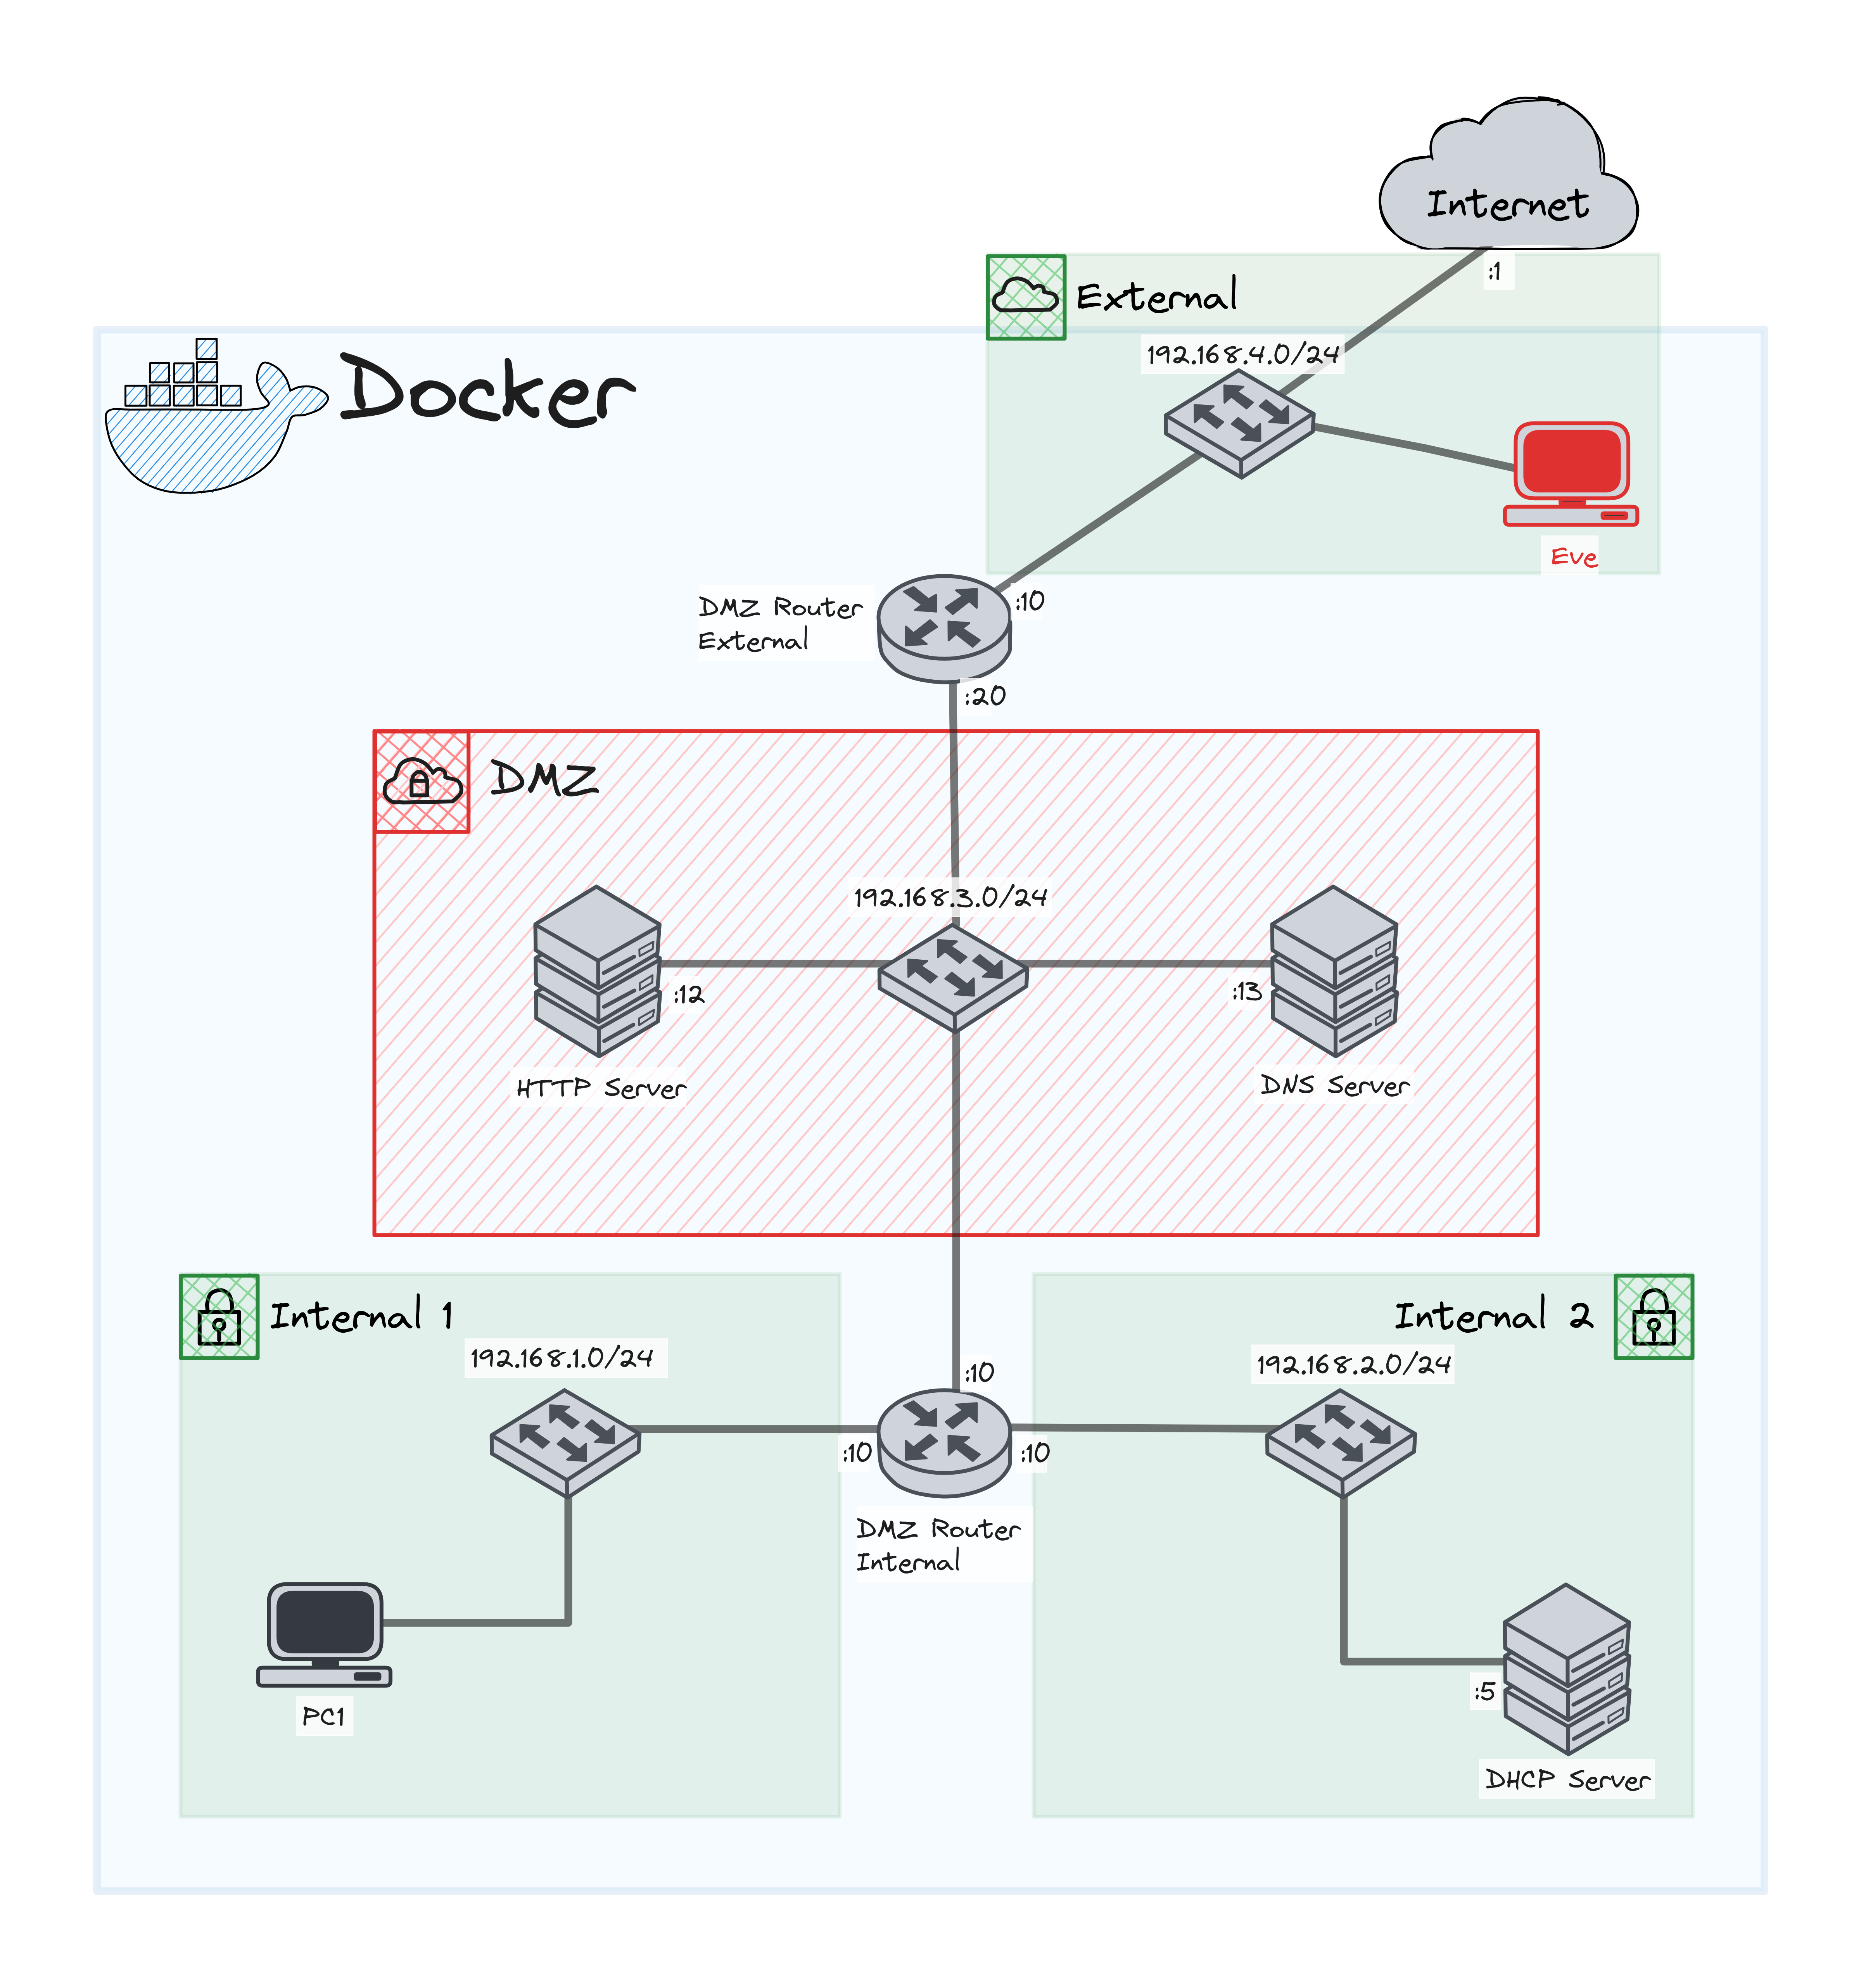
\includegraphics{Images/Diagram1.png}
\newpage

\section{Firewalls and Routing}\label{firewalls-and-routing}

For this project, we are using Ubuntu based routers with
\texttt{iptables} for firewall and NAT, and \texttt{ip\ route} for
routing. Because the container we provided have system capabilities to
forward the ipv4 packets, they act like a router.

\subsection{IPTables}\label{iptables}

\subsubsection{Setting rules}\label{setting-rules}

\texttt{iptables} is powerful tool to manage firewall rules on a linux
system, as it is only CLI, it is widely used on servers. The
\texttt{iptables} have three main categories:

\begin{itemize}
\tightlist
\item
  INPUT
\item
  FORWARD
\item
  OUTPUT
\end{itemize}

In this docker simulation, we use only FORWARD rules for firewall.
Therefore, we will mainly set only such rules during the exercises, but
the rules are almost identical between categories.

\paragraph{Questions}\label{questions}

\begin{enumerate}
\def\labelenumi{\arabic{enumi}.}
\tightlist
\item
  Connect to DMZ\_Router\_External and find a way to print the firewall
  rules. Optionnal: Print detailed firewall rules.
\item
  Show the NAT rules set in iptables
\item
  Create an INPUT rule to allow http service
\end{enumerate}

\newpage

\paragraph{Answers}\label{answers}

\begin{enumerate}
\def\labelenumi{\arabic{enumi}.}
\item
  To show the firewall rules on the router, we can use the command
  \texttt{iptables\ -L}, and if we want detailed rules, we can upgrade
  the verbosity using \texttt{-v}:

  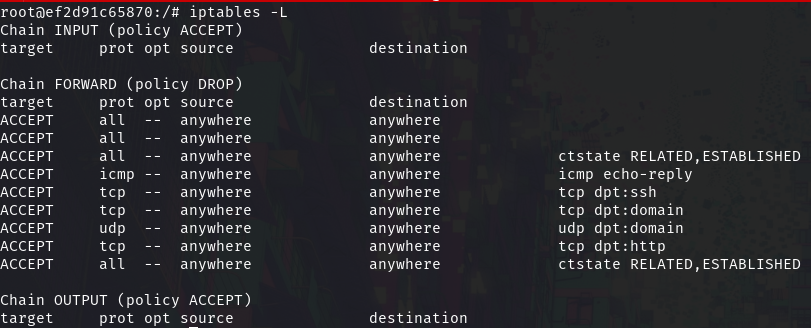
\includegraphics{Images/Image01.png}

  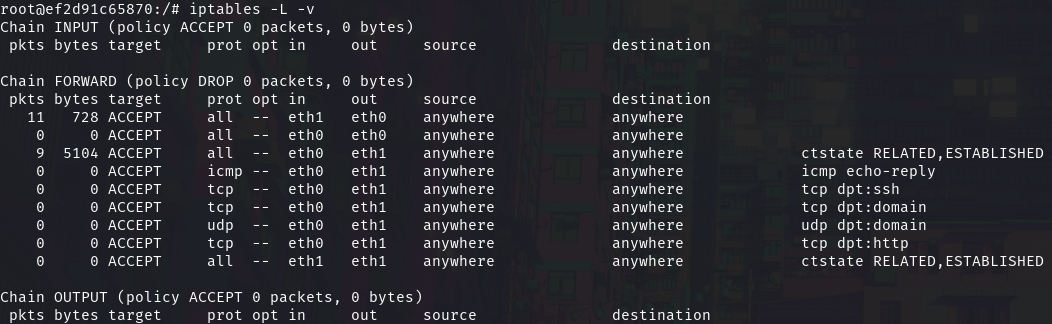
\includegraphics{Images/Image02.png}
\item
  The NAT rules are not showed with previous command, you need to add
  the parameter \texttt{-t\ nat}. Which will print the nat rules like
  follow:

  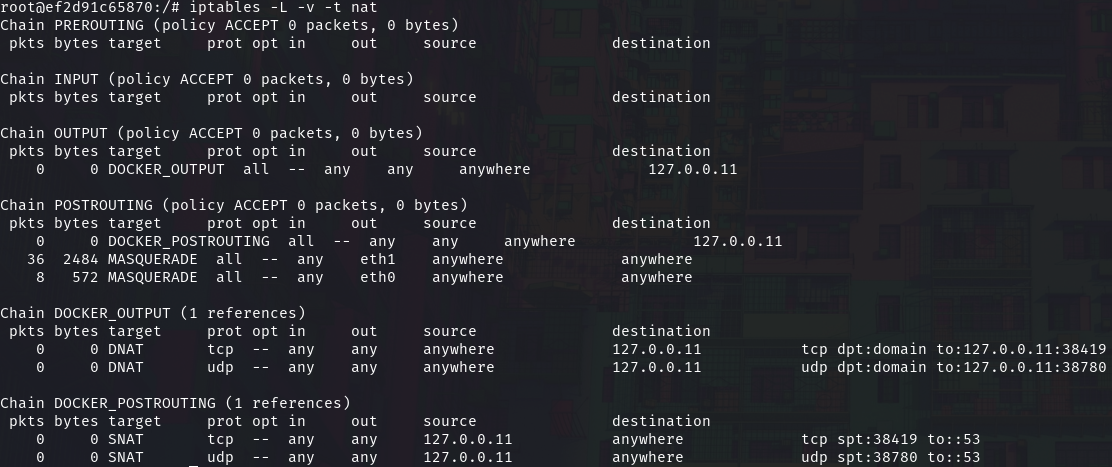
\includegraphics{Images/Image03.png}
  The \texttt{DOCKER\_*} categories are specific to the setup
  environment, meaning you won't normally find it anywere else. We can
  see that \texttt{POSTROUTING} is set on the interfaces of the router,
  meaning we have NAT rules !

\newpage
  
\item
  To create an INPUT to allow http service, you need to run the
  following:

\begin{Shaded}
\begin{Highlighting}[]
    \ExtensionTok{iptables} \AttributeTok{{-}A}\NormalTok{ INPUT }\AttributeTok{{-}p}\NormalTok{ tcp }\AttributeTok{{-}{-}dport}\NormalTok{ 80 }\AttributeTok{{-}j}\NormalTok{ ACCEPT}
\end{Highlighting}
\end{Shaded}

  Explanation of the options used:

  \begin{itemize}
  \tightlist
  \item
    \texttt{-A\ INPUT}: Appends a rule to the INPUT chain.
  \item
    \texttt{-p\ tcp}: Specifies the protocol as TCP.
  \item
    \texttt{-\/-dport\ 80}: Specifies the destination port as 80 (HTTP).
  \item
    \texttt{-j\ ACCEPT}: Specifies the target action as ACCEPT. You can
    use the command from question 1 to see if the rule is set !
  \end{itemize}
\end{enumerate}

\subsubsection{Setting a stateful
firewall}\label{setting-a-stateful-firewall}

If you check again the output of \texttt{iptables\ -L}, you might notice
that some rules have a \texttt{ctstate} writen. This meaning that the
firewall will be applying a stateful rule using \texttt{conntrack}.
Connection tracking is the main difference between what we call a
stateless firewall and a stateful firewall.

With a stateless firewall, when a connection is esthablished, the
firewall will check its source and destination, go through the firewall
rules and then allow the connection. But with a stateful firewall, the
firewall will keep track of the connection state and therefore detect if
it is a new connection attempt or a part of an established one.

The stateful firewall is more secured and has better performance,
therefore it is recommended to use it ! With \texttt{iptables}, it is
very simple to set a stateful rule, we just need to add the parameter
\texttt{-\/-cstate\ \textless{}flag\textgreater{}}. Usually, we use the
flags \texttt{ESTABLISHED}, \texttt{NEW} or \texttt{RELATED}.

Let's change the http rule we had set before, to do so, we need to first
delete the input rule we made:

\begin{Shaded}
\begin{Highlighting}[]
\ExtensionTok{iptables} \AttributeTok{{-}D}\NormalTok{ INPUT 1}
\end{Highlighting}
\end{Shaded}

Then, we add the flags \texttt{ESTABLISHED} and \texttt{NEW}, which will
allow us to create new connection but also to track the established
ones:

\begin{Shaded}
\begin{Highlighting}[]
    \ExtensionTok{iptables} \AttributeTok{{-}A}\NormalTok{ INPUT }\AttributeTok{{-}p}\NormalTok{ tcp }\AttributeTok{{-}{-}dport}\NormalTok{ 80 }\AttributeTok{{-}m}\NormalTok{ conntrack }\AttributeTok{{-}{-}ctstate}\NormalTok{ NEW,ESTABLISHED }\AttributeTok{{-}j}\NormalTok{ ACCEPT}
\end{Highlighting}
\end{Shaded}

\subsubsection{Save rules}\label{save-rules}

All the rules we have set since now are not persistent, meaning that if
the machine restart, it will be lost. Therefore, they many ways to save
them and restore them, but we will detail one.

\begin{enumerate}
\def\labelenumi{\arabic{enumi}.}
\tightlist
\item
  Save the rules in a file using
  \texttt{iptables-save\ \textgreater{}\ /etc/iptables/rules.v4}
\item
  Set a cron task at reboot that will run the following
  \texttt{iptables-restore\ \textless{}\ /etc/iptables/rules.v4}
\end{enumerate}

Therefore, using \texttt{iptables-save} and \texttt{iptables-restore},
you can backup and restore your configuration. If you make a mistake of
configuration or you are doing some testing, this is very useful in
order to avoid service disruptions.

\subsection{IP routes}\label{ip-routes}

In order to some routing on ubuntu system, we decided to use
\texttt{ip\ route}. This set of command is helpful to set route path to
subnets, the default gateway, get stats from a route path and so on.

First of all, we will show the \texttt{ip\ route} set on the
DMZ\_Router\_External, let's connect to it and run the following:

\begin{Shaded}
\begin{Highlighting}[]
\ExtensionTok{ip}\NormalTok{ route show}
\end{Highlighting}
\end{Shaded}

Here is the result:
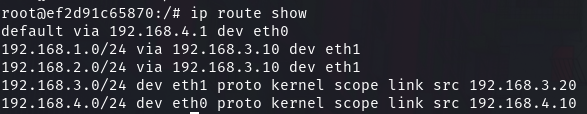
\includegraphics{Images/Image04.png}

\subsubsection{Questions}\label{questions-1}

\begin{enumerate}
\def\labelenumi{\arabic{enumi}.}
\tightlist
\item
  What is the default gateway on the router ?
\item
  Which interface is used to access the subnet \texttt{192.168.3.0/24} ?
\item
  Find a way to show the ip address of the machine
\end{enumerate}

\newpage

\subsubsection{Answers}\label{answers-1}

\begin{enumerate}
\def\labelenumi{\arabic{enumi}.}
\item
  The default gateway is written on the first line as
  \texttt{default\ via\ 192.168.4.1\ dev\ eth0}. Which means that
  \texttt{192.168.4.1} is the default gateway address of the router and
  is located on interface \texttt{eth0}.
\item
  Reading the output of \texttt{ip\ route\ show}, we can see that the
  interface responsible of \texttt{192.168.3.0/24} is \texttt{eth1}. We
  can see for other subnets that the path is specified \texttt{via},
  which means it will get to an IP address to reach the requested
  subnet!
\item
  In order to show the ip address of the machine, you can simply run
  \texttt{ip\ a}

  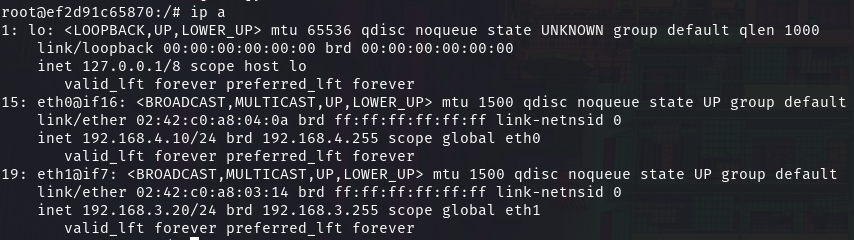
\includegraphics{Images/Image05.png}
  You can read the ip address on \texttt{inet} for each interface ! You
  can even read the MAC address on \texttt{link/ether}.
\end{enumerate}

\subsection{Troubleshooting}\label{troubleshooting}

IP routes are not parameters that you will set a lot. Usually you set
them once at the initial setup and that's it, you might update them if
you changed your router config but it is rare. Also, on sophisticated
routers, you don't even need to go on each machines to set the ip routes
because they will provide them. On our setup, we had to set them as we
are in a docker environment.

The gateway will be set either manually, either by the DHCP server,
therefore mistakes can happen. If you notice issues in terms of
connections, you can try to ping networks using
\texttt{ping\ \textless{}ip\textgreater{}}. But also using ip routes,
you can see if the route is cached or not, using
\texttt{ip\ route\ get\ \textless{}ip\textgreater{}}. This command is
similar to \texttt{traceroute\ \textless{}ip\textgreater{}}.

Let's try the previous commands on the DMZ\_Router\_External.

One issue can be a missing route to a network, to add them, you can run
\texttt{ip\ route\ add\ {[}destination{]}\ via\ {[}gatewayIP{]}}. And to
delete them
\texttt{ip\ route\ del\ {[}destination{]}\ via\ {[}gatewayIP{]}}. If you
wanna change the default gateway, simply run
\texttt{ip\ route\ add\ default\ via\ {[}gateway{]}}.

\section{Services}\label{services}

In this docker simulation, we are a running three main services: web
server, a domain name server and a DHCP server.

\subsection{HTTP}\label{http}

This server is hosting an HTTP server running a javascript website using
NodeJS. Therefore, we can see the service running using different
commands.

At first, we see if the port 80 is currently used using
\texttt{ss\ -tlpn}:

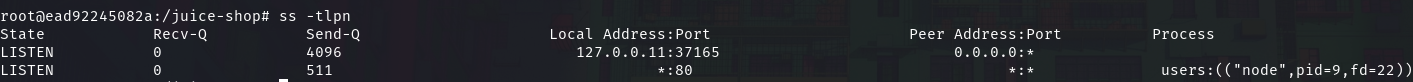
\includegraphics{Images/Image06.png}

We can read a state LISTEN on the port \texttt{*:80} , we can even read
the Process ID of node. Speaking of process, we can check if the process
is running fine using \texttt{ps\ -aux}:

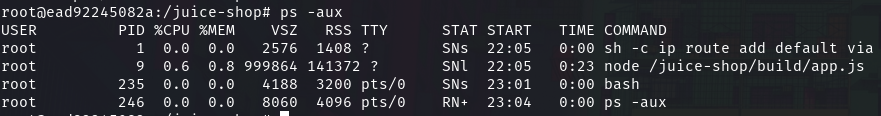
\includegraphics{Images/Image07.png}
Therefore we can see which command was used to start the website ! And
also, we can use \texttt{kill\ \textless{}pid\textgreater{}} to stop the
service from running. But as we can read the command, we can simply
restart it.

If you want a more interactive way to show the process, you can run
\texttt{top} command.

\subsubsection{Question}\label{question}

\begin{enumerate}
\def\labelenumi{\arabic{enumi}.}
\tightlist
\item
  Can you find the logs related to the access of the website ?
\end{enumerate}

\newpage

\subsubsection{Answers}\label{answers-2}

\begin{enumerate}
\def\labelenumi{\arabic{enumi}.}
\item
  In order to find the logs, we can run an \texttt{ls} command in the
  folder \texttt{/juice-shop} and notice a folder called \texttt{logs}
  containing the requested logs. But what if we wanted to find them
  located in another folder ? We can run a
  \texttt{find\ /\ -name\ "*access*log*"} in order to find them !

  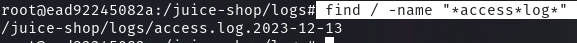
\includegraphics{Images/Image08.png}
\end{enumerate}

\subsection{DNS}\label{dns}

As you can see on the diagram of the project, we have a DNS server
inside the DMZ. Therefore, we will use its configuration files in order
to understand how it is set!

\subsubsection{Bind9}\label{bind9}

To have a DNS server, we need a service and to do so, we use Bind9, also
called ``named''. Using the \texttt{ps\ -aux} or \texttt{top} commands,
you can see it running !

The DNS configuration files will be stored in \texttt{/etc/bind/} :

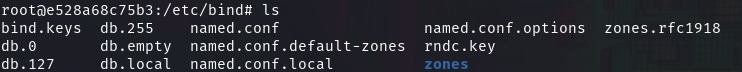
\includegraphics{Images/Image09.png}

In this folder we need to focus on three files at the moment:

\begin{itemize}
\tightlist
\item
  \texttt{named.conf.options}
\item
  \texttt{named.conf.local}
\item
  \texttt{/zones/juice-shop.local}
\end{itemize}

Each file ending on \texttt{.local} is a zone file, which will be
detailed in the next part ! Let's read the content of
\texttt{named.conf.options} using \texttt{cat}:

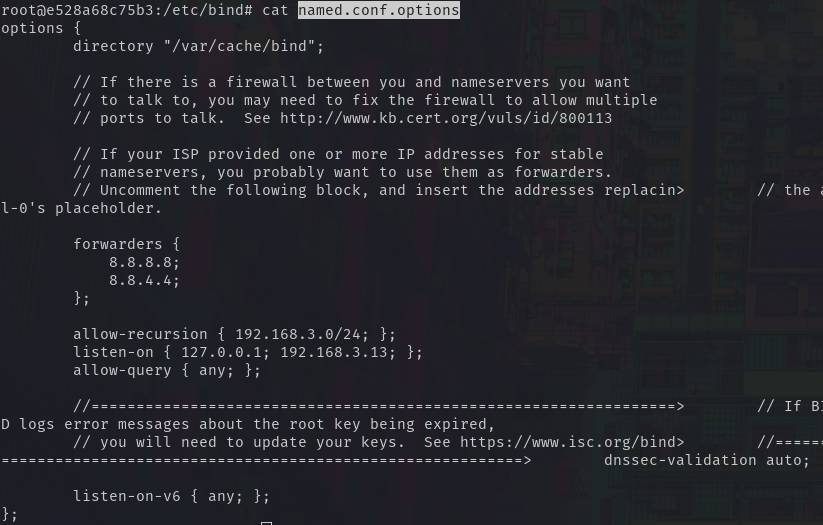
\includegraphics{Images/Image10.png}

Here, we can read the options currently set for the DNS server we are
running. One of the most important option is \texttt{forwarders} because
it allows the DNS server to query another DNS server if the request
domain isn't known.

\paragraph{Questions}\label{questions-2}

\begin{enumerate}
\def\labelenumi{\arabic{enumi}.}
\tightlist
\item
  Find who's forwarder is \texttt{8.8.8.8}
\item
  Find another famous forwarder and set it. How can you restart the
  service for the setting to apply ?
\end{enumerate}

\newpage

\paragraph{Answers}\label{answers-3}

\begin{enumerate}
\def\labelenumi{\arabic{enumi}.}
\item
  \texttt{8.8.8.8} is the DNS of google !
\item
  Another famous is DNS is \texttt{1.1.1.1}. After editing the file
  using \texttt{vim}, you can restart the service using
  \texttt{service\ named\ restart}:

  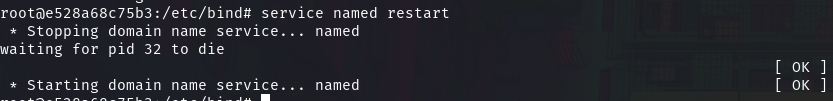
\includegraphics{Images/Image11.png}
  As you can read \texttt{{[}\ OK\ {]}}, it means the service restarted
  properly and you didn't made any mistake on the forwarder change !
\end{enumerate}

\subsubsection{Zones}\label{zones}

In the context of DNS, a zone refers to a portion of the domain
namespace for which a particular DNS server is responsible. Each zone
contains information about the domain names within that space and their
associated resource records.

Let's explore the contents of the \texttt{named.conf.local} file to
understand how zones are configured. Use the \texttt{cat} command to
view the file:

\begin{Shaded}
\begin{Highlighting}[]
\FunctionTok{cat}\NormalTok{ /etc/bind/named.conf.local}
\end{Highlighting}
\end{Shaded}

This file typically includes statements for defining zone
configurations:

\begin{Shaded}
\begin{Highlighting}[]
\ExtensionTok{zone} \StringTok{"juiceshop.local"}\NormalTok{ \{}
    \BuiltInTok{type}\NormalTok{ master}\KeywordTok{;}
    \FunctionTok{file} \StringTok{"/etc/bind/zones/juiceshop.local"}\KeywordTok{;}
\ErrorTok{\}}\KeywordTok{;}
\end{Highlighting}
\end{Shaded}

This snippet indicates that there is a zone named ``juiceshop.local,''
and the associated information is stored in the file
\texttt{/etc/bind/zones/juiceshop.local}. The \texttt{type\ master;}
statement signifies that this DNS server is authoritative for the zone.

Now, let's examine the contents of a sample zone file, such as
\texttt{/etc/bind/zones/juiceshop.local}. You can use the \texttt{cat}
command to display the file:

\begin{Shaded}
\begin{Highlighting}[]
\FunctionTok{cat}\NormalTok{ /etc/bind/zones/juice{-}shop.local}
\end{Highlighting}
\end{Shaded}

A zone file typically includes various resource records (RRs) that
provide information about the domain. Common types of RRs include:

\begin{itemize}
\tightlist
\item
  \textbf{SOA (Start of Authority):} Provides authoritative information
  about the domain and the zone.
\item
  \textbf{NS (Name Server):} Specifies authoritative DNS servers for the
  domain.
\item
  \textbf{A (Address):} Maps a domain to an IPv4 address.
\item
  \textbf{AAAA (IPv6 Address):} Maps a domain to an IPv6 address.
\item
  \textbf{CNAME (Canonical Name):} Creates an alias for a domain.
\item
  \textbf{MX (Mail Exchange):} Specifies mail servers for the domain.
\end{itemize}

\newpage

Here's the zone file of juiceshop:

\begin{Shaded}
\begin{Highlighting}[]
\VariableTok{$TTL}\NormalTok{ 1D}
\ExtensionTok{@}\NormalTok{       IN      SOA     ns1.juiceshop.local. admin.juiceshop.local. }\ErrorTok{(}
                \ExtensionTok{2023111601} \KeywordTok{;} \ExtensionTok{Serial}
                \ExtensionTok{3H} \KeywordTok{;} \ExtensionTok{Refresh}
                \ExtensionTok{15} \KeywordTok{;} \ExtensionTok{Retry}
                \ExtensionTok{1w} \KeywordTok{;} \ExtensionTok{Expire}
                \ExtensionTok{3h} \KeywordTok{;} \ExtensionTok{Negative}\NormalTok{ Cache TTL}
\KeywordTok{);}

\ExtensionTok{@}\NormalTok{       IN      NS      ns1.juiceshop.local.}
\ExtensionTok{@}\NormalTok{       IN      A       192.168.3.12}
\ExtensionTok{www}\NormalTok{     IN      A       192.168.3.12}
\ExtensionTok{ns1}\NormalTok{     IN      A       192.168.3.13}
\end{Highlighting}
\end{Shaded}

\paragraph{Question}\label{question-1}

\begin{enumerate}
\def\labelenumi{\arabic{enumi}.}
\tightlist
\item
  Create a zone for \texttt{example.com} and use
  \texttt{traceroute\ example.com} to show the proper configuration.
\end{enumerate}

\newpage

\paragraph{Answer}\label{answer}

\begin{enumerate}
\def\labelenumi{\arabic{enumi}.}
\item
  To create zone for example.com, you first need to create a zone file :

\begin{Shaded}
\begin{Highlighting}[]
    \FunctionTok{nano}\NormalTok{ /etc/bind/zones/example.com}
\end{Highlighting}
\end{Shaded}

  Then you will edit the file as follow:

\begin{Shaded}
\begin{Highlighting}[]
    \VariableTok{$TTL}\NormalTok{ 1D}
    \ExtensionTok{@}\NormalTok{       IN      SOA     ns1.example.com. admin.example.com. }\ErrorTok{(}
                    \ExtensionTok{2023111601} \KeywordTok{;} \ExtensionTok{Serial}
                    \ExtensionTok{3H} \KeywordTok{;} \ExtensionTok{Refresh}
                    \ExtensionTok{15} \KeywordTok{;} \ExtensionTok{Retry}
                    \ExtensionTok{1w} \KeywordTok{;} \ExtensionTok{Expire}
                    \ExtensionTok{3h} \KeywordTok{;} \ExtensionTok{Negative}\NormalTok{ Cache TTL}
    \KeywordTok{);}

    \ExtensionTok{@}\NormalTok{       IN      NS      ns1.example.com.}
    \ExtensionTok{@}\NormalTok{       IN      A       192.168.4.3}
    \ExtensionTok{www}\NormalTok{     IN      A       192.168.4.3}
    \ExtensionTok{ns1}\NormalTok{     IN      A       192.168.4.3}
\end{Highlighting}
\end{Shaded}

  Saving and exiting the file, you will now add the zone entry into
  \texttt{/etc/bind/named.conf.local}

\begin{Shaded}
\begin{Highlighting}[]
    \ExtensionTok{zone} \StringTok{"example.com"}\NormalTok{ \{}
        \BuiltInTok{type}\NormalTok{ master}\KeywordTok{;}
        \FunctionTok{file} \StringTok{"/etc/bind/zones/example.com"}\KeywordTok{;}
    \ErrorTok{\}}\KeywordTok{;}
\end{Highlighting}
\end{Shaded}

  Now you just have to restart the service using
  \texttt{service\ named\ restart} and check the output of
  \texttt{traceroute\ example.com}:

  
\includegraphics{Images/Image12.png}

  The IP is the one we have set into the DNS configuration, therefore it
  is now working !
\end{enumerate}

\subsection{DHCP}\label{dhcp}

If you pay attention to the diagram, you might see that the DHCP server
is not located into the DMZ, because it should not be accessible from
the outside ! Therefore, we have less strict firewall rules when
accessing PC1 from DHCP server.

The DHCP server will be using package called \texttt{isc-dhcp-server},
which we will be the DHCP service ! It has two main files:

\begin{itemize}
\tightlist
\item
  \texttt{/etc/dhcp/dhcpd.conf}
\item
  \texttt{/etc/default/isc-dhcp-server}
\end{itemize}

Let's start with \texttt{/etc/default/isc-dhcp-server}, check its
content using \texttt{cat} command.

\begin{Shaded}
\begin{Highlighting}[]
\VariableTok{INTERFACESv4}\OperatorTok{=}\StringTok{"eth0"}
\VariableTok{INTERFACESv6}\OperatorTok{=}\StringTok{""}
\end{Highlighting}
\end{Shaded}

You might notice a lot of comments and only one parameter set. This
parameter specify which interface the DHCP server should listen for DHCP
requests of new devices!

Now, let's check \texttt{/etc/dhcp/dhcpd.conf} with \texttt{cat}
command:

\begin{Shaded}
\begin{Highlighting}[]
\CommentTok{\# option definitions common to all supported network}
\ExtensionTok{subnet}\NormalTok{ 192.168.2.0 netmask 255.255.255.0 \{}
\ErrorTok{\}}
\ExtensionTok{subnet}\NormalTok{ 192.168.1.0 netmask 255.255.255.0 \{}
    \ExtensionTok{range}\NormalTok{ 192.168.1.2 192.168.1.20}\KeywordTok{;}
    \ExtensionTok{option}\NormalTok{ routers 192.168.1.10}\KeywordTok{;}
    \ExtensionTok{option}\NormalTok{ domain{-}name{-}servers 192.168.3.13}\KeywordTok{;}
    \ExtensionTok{option}\NormalTok{ domain{-}name }\StringTok{"dockersec.com"}\KeywordTok{;} 
    \ExtensionTok{option}\NormalTok{ broadcast{-}address 192.168.1.255}\KeywordTok{;}
    \ExtensionTok{default{-}lease{-}time}\NormalTok{ 600}\KeywordTok{;}
    \ExtensionTok{max{-}lease{-}time}\NormalTok{ 7200}\KeywordTok{;}
\ErrorTok{\}}
\end{Highlighting}
\end{Shaded}

Once again, you might notice plenty of comments, but let's focus on this
part. As you can see we have two subnets with a netmask. From the
different options on \texttt{192.168.1.0}, we can read the following:

\begin{itemize}
\tightlist
\item
  \texttt{range\ 192.168.1.2\ 192.168.1.20;} --\textgreater{} this is
  the IP range we will give to the devices connecting to this subnet.
\item
  \texttt{option\ routers\ 192.168.1.10;} --\textgreater{} that will
  define the default gateway of the device.
\item
  \texttt{option\ domain-name-servers\ 192.168.3.13;} \&
  \texttt{option\ domain-name\ "dockersec.com";} --\textgreater{} these
  are responsible of the DNS configuration and will specify the DNS
  server IP and name !
\item
  \texttt{option\ broadcast-address\ 192.168.1.255;} --\textgreater{} we
  need to know which ip to use for broadcasts.
\item
  \texttt{default-lease-time\ 600;} \& \texttt{max-lease-time\ 7200;}
  --\textgreater{} this will define in seconds how long a DHCP lease
  will be set for, so how long our device will have the IP set.
\end{itemize}

\subsubsection{Questions}\label{questions-3}

\begin{enumerate}
\def\labelenumi{\arabic{enumi}.}
\tightlist
\item
  How can you extend the IP range from 19 IPs to 40 ?
\item
  How to restart the service ?
\end{enumerate}

\newpage

\subsubsection{Answers}\label{answers-4}

\begin{enumerate}
\def\labelenumi{\arabic{enumi}.}
\item
  To extend the IP range, you need to change the ligne
  \texttt{range\ 192.168.1.2\ 192.168.1.20;} to
  \texttt{range\ 192.168.1.2\ 192.168.1.41;} for example.
\item
  You need to run \texttt{service\ isc-dhcp-server\ restart} :

  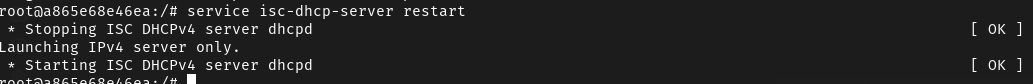
\includegraphics{Images/Image13.png}
\end{enumerate}

\end{document}